\ifx\allfiles\undefined
\documentclass[12pt, a4paper, oneside, UTF8]{ctexbook}
\def\path{../config}
\usepackage{amsmath}
\usepackage{amsthm}
\usepackage{array}
\usepackage{amssymb}
\usepackage{graphicx}
\usepackage{mathrsfs}
\usepackage{enumitem}
\usepackage{geometry}
\usepackage[colorlinks, linkcolor=black]{hyperref}
\usepackage{stackengine}
\usepackage{yhmath}
\usepackage{extarrows}
% \usepackage{unicode-math}
\usepackage{esint}
\usepackage{multirow}
\usepackage{fancyhdr}
\usepackage[dvipsnames, svgnames]{xcolor}
\usepackage{listings}
\usepackage{float} % Required for the H float option
\definecolor{mygreen}{rgb}{0,0.6,0}
\definecolor{mygray}{rgb}{0.5,0.5,0.5}
\definecolor{mymauve}{rgb}{0.58,0,0.82}
\definecolor{NavyBlue}{RGB}{0,0,128}
\definecolor{Rhodamine}{RGB}{255,0,255}
\definecolor{PineGreen}{RGB}{0,128,0}

\graphicspath{ {figures/},{../figures/}, {config/}, {../config/} }

\linespread{1.6}

\geometry{
    top=25.4mm, 
    bottom=25.4mm, 
    left=20mm, 
    right=20mm, 
    headheight=2.17cm, 
    headsep=4mm, 
    footskip=12mm
}

\setenumerate[1]{itemsep=5pt,partopsep=0pt,parsep=\parskip,topsep=5pt}
\setitemize[1]{itemsep=5pt,partopsep=0pt,parsep=\parskip,topsep=5pt}
\setdescription{itemsep=5pt,partopsep=0pt,parsep=\parskip,topsep=5pt}

\lstset{
    language=Mathematica,
    basicstyle=\tt,
    breaklines=true,
    keywordstyle=\bfseries\color{NavyBlue}, 
    emphstyle=\bfseries\color{Rhodamine},
    commentstyle=\itshape\color{black!50!white}, 
    stringstyle=\bfseries\color{PineGreen!90!black},
    columns=flexible,
    numbers=left,
    numberstyle=\footnotesize,
    frame=tb,
    breakatwhitespace=false,
} 

\lstset{
    language=TeX, % 设置语言为 TeX
    basicstyle=\ttfamily, % 使用等宽字体
    breaklines=true, % 自动换行
    keywordstyle=\bfseries\color{NavyBlue}, % 关键字样式
    emphstyle=\bfseries\color{Rhodamine}, % 强调样式
    commentstyle=\itshape\color{black!50!white}, % 注释样式
    stringstyle=\bfseries\color{PineGreen!90!black}, % 字符串样式
    columns=flexible, % 列的灵活性
    numbers=left, % 行号在左侧
    numberstyle=\footnotesize, % 行号字体大小
    frame=tb, % 顶部和底部边框
    breakatwhitespace=false % 不在空白处断行
}

% \begin{lstlisting}[language=TeX] ... \end{lstlisting}

% 定理环境设置
\usepackage[strict]{changepage} 
\usepackage{framed}

\definecolor{greenshade}{rgb}{0.90,1,0.92}
\definecolor{redshade}{rgb}{1.00,0.88,0.88}
\definecolor{brownshade}{rgb}{0.99,0.95,0.9}
\definecolor{lilacshade}{rgb}{0.95,0.93,0.98}
\definecolor{orangeshade}{rgb}{1.00,0.88,0.82}
\definecolor{lightblueshade}{rgb}{0.8,0.92,1}
\definecolor{purple}{rgb}{0.81,0.85,1}

\theoremstyle{definition}
\newtheorem{myDefn}{\indent Definition}[section]
\newtheorem{myLemma}{\indent Lemma}[section]
\newtheorem{myThm}[myLemma]{\indent Theorem}
\newtheorem{myCorollary}[myLemma]{\indent Corollary}
\newtheorem{myCriterion}[myLemma]{\indent Criterion}
\newtheorem*{myRemark}{\indent Remark}
\newtheorem{myProposition}{\indent Proposition}[section]

\newenvironment{formal}[2][]{%
	\def\FrameCommand{%
		\hspace{1pt}%
		{\color{#1}\vrule width 2pt}%
		{\color{#2}\vrule width 4pt}%
		\colorbox{#2}%
	}%
	\MakeFramed{\advance\hsize-\width\FrameRestore}%
	\noindent\hspace{-4.55pt}%
	\begin{adjustwidth}{}{7pt}\vspace{2pt}\vspace{2pt}}{%
		\vspace{2pt}\end{adjustwidth}\endMakeFramed%
}

\newenvironment{definition}{\vspace{-\baselineskip * 2 / 3}%
	\begin{formal}[Green]{greenshade}\vspace{-\baselineskip * 4 / 5}\begin{myDefn}}
	{\end{myDefn}\end{formal}\vspace{-\baselineskip * 2 / 3}}

\newenvironment{theorem}{\vspace{-\baselineskip * 2 / 3}%
	\begin{formal}[LightSkyBlue]{lightblueshade}\vspace{-\baselineskip * 4 / 5}\begin{myThm}}%
	{\end{myThm}\end{formal}\vspace{-\baselineskip * 2 / 3}}

\newenvironment{lemma}{\vspace{-\baselineskip * 2 / 3}%
	\begin{formal}[Plum]{lilacshade}\vspace{-\baselineskip * 4 / 5}\begin{myLemma}}%
	{\end{myLemma}\end{formal}\vspace{-\baselineskip * 2 / 3}}

\newenvironment{corollary}{\vspace{-\baselineskip * 2 / 3}%
	\begin{formal}[BurlyWood]{brownshade}\vspace{-\baselineskip * 4 / 5}\begin{myCorollary}}%
	{\end{myCorollary}\end{formal}\vspace{-\baselineskip * 2 / 3}}

\newenvironment{criterion}{\vspace{-\baselineskip * 2 / 3}%
	\begin{formal}[DarkOrange]{orangeshade}\vspace{-\baselineskip * 4 / 5}\begin{myCriterion}}%
	{\end{myCriterion}\end{formal}\vspace{-\baselineskip * 2 / 3}}
	

\newenvironment{remark}{\vspace{-\baselineskip * 2 / 3}%
	\begin{formal}[LightCoral]{redshade}\vspace{-\baselineskip * 4 / 5}\begin{myRemark}}%
	{\end{myRemark}\end{formal}\vspace{-\baselineskip * 2 / 3}}

\newenvironment{proposition}{\vspace{-\baselineskip * 2 / 3}%
	\begin{formal}[RoyalPurple]{purple}\vspace{-\baselineskip * 4 / 5}\begin{myProposition}}%
	{\end{myProposition}\end{formal}\vspace{-\baselineskip * 2 / 3}}


\newtheorem{example}{\indent \color{SeaGreen}{Example}}[section]
\renewcommand{\proofname}{\indent\textbf{\textcolor{TealBlue}{Proof}}}
\newenvironment{solution}{\begin{proof}[\indent\textbf{\textcolor{TealBlue}{Solution}}]}{\end{proof}}

% 自定义命令的文件

\def\d{\mathrm{d}}
\def\R{\mathbb{R}}
%\newcommand{\bs}[1]{\boldsymbol{#1}}
%\newcommand{\ora}[1]{\overrightarrow{#1}}
\newcommand{\myspace}[1]{\par\vspace{#1\baselineskip}}
\newcommand{\xrowht}[2][0]{\addstackgap[.5\dimexpr#2\relax]{\vphantom{#1}}}
\newenvironment{mycases}[1][1]{\linespread{#1} \selectfont \begin{cases}}{\end{cases}}
\newenvironment{myvmatrix}[1][1]{\linespread{#1} \selectfont \begin{vmatrix}}{\end{vmatrix}}
\newcommand{\tabincell}[2]{\begin{tabular}{@{}#1@{}}#2\end{tabular}}
\newcommand{\pll}{\kern 0.56em/\kern -0.8em /\kern 0.56em}
\newcommand{\dive}[1][F]{\mathrm{div}\;\boldsymbol{#1}}
\newcommand{\rotn}[1][A]{\mathrm{rot}\;\boldsymbol{#1}}

% 修改参数改变封面样式,0 默认原始封面、内置其他1、2、3种封面样式
\def\myIndex{0}


\ifnum\myIndex>0
    \input{\path/cover_package_\myIndex}
\fi

\def\myTitle{标题:一份LaTeX笔记模板}
\def\myAuthor{作者名称}
\def\myDateCover{封面日期: \today}
\def\myDateForeword{前言页显示日期: \today}
\def\myForeword{前言标题}
\def\myForewordText{
    
    这是一个基于\LaTeX{}的模板,用于撰写学习笔记。

    模板旨在提供一个简单、易用的框架,以便你能够专注于内容,而不是排版细节,如不是专业者,不建议使用者在模板细节上花费太多时间,而是直接使用模板进行笔记撰写。遇到问题,再进行调整解决。
}
\def\mySubheading{副标题}


\begin{document}
\input{\path/cover_text_\myIndex.tex}

\newpage
\thispagestyle{empty}
\begin{center}
    \Huge\textbf{\myForeword}
\end{center}
\myForewordText
\begin{flushright}
    \begin{tabular}{c}
        \myDateForeword
    \end{tabular}
\end{flushright}

\newpage
\pagestyle{plain}
\setcounter{page}{1}
\pagenumbering{Roman}
\tableofcontents

\newpage
\pagenumbering{arabic}
\setcounter{chapter}{-1}
\setcounter{page}{1}

\pagestyle{fancy}
\fancyfoot[C]{\thepage}
\renewcommand{\headrulewidth}{0.4pt}
\renewcommand{\footrulewidth}{0pt}








\else
\fi

\chapter{风荷载}

\begin{theorem}
$$
w = w_m - w_b = \frac{1}{2} \rho v^2 = \frac{1}{2} \frac{\gamma}{g} v^2
$$

风速与风压的关系公式,其中 $w_m$为最大风压力(速度降为0),$w_b$为原先风压力,$\gamma$ 为空气单位体积的重力,$g$ 为重力加速度。
\end{theorem}

基本风压的相关因素:

\begin{enumerate}
    \item 地貌(影响摩擦)
    \item 标高(一般取10m)
    \item 最大风速的样本时间:样本时间显然越长越大
    \item 公称风速的时距:公称风速实际是一定时间间隔的平均风速,不可过长也不可过短。
    \item 基本风速重现期的长短:{\color{red}该时间范围内的最大风速定义为基本风速}
\end{enumerate}

\begin{definition}
    根据实测结果分析,平均风速沿高度变化的规律可用指数函数来描述,即

$$
\frac{\bar{v}}{v_s} = \left( \frac{z}{z_s} \right)^\alpha
$$

式中 $\bar{v}$、$z$——任一点的平均风速和高度;

$v_s$、$z_s$——标准高度处的平均风速和高度(一般取10m)。

$\alpha$——与地貌或地面粗糙度有关的指数。
\end{definition}

由于远离地面的高度的风速相同,$$v_{0s} \left( \frac{H_{Ts}}{z_s} \right)^{\alpha_s} = v_{0a} \left( \frac{H_{Ta}}{z_a} \right)^{\alpha_a}$$
于是有
\[
v_{0a} = v_{0s} \left( \frac{H_{Ts}}{z_s} \right)^{\alpha_s} \left( \frac{H_{Ta}}{z_a} \right)^{-\alpha_a} 
\]

可得任意地貌的基本风压 \(w_{0a}\) 与标准地貌的基本风压 \(w_0\) 的关系为:

\[
w_{0a} = w_{0s} \left( \frac{H_{Ts}}{z_s} \right)^{2\alpha_s} \left( \frac{H_{Ta}}{z_a} \right)^{-2\alpha_a} 
\]

不同地表粗糙度有不同的梯度风高度,地面粗糙度小,风速变化快,梯度风高度比地面粗糙度大的地区低;反之,地面粗糙度越大,梯度风高度将越高。

\begin{remark}
    任一水平风作用在任意截面的细长物体表面上,会在其表面产生风压,将物体表面上的风压沿表面积分,将得到三种力的成分,即顺风向力 \( P_D \)、横风向力 \( P_L \) 及扭力矩 \( P_M \)。
    
    顺风向的风效应分解为平均风 (即稳定风)和脉动风(也称阵风脉动)。

    横风向力较顺风向力小得多,对于对称结构,横风向力更是可以忽略。
    然而,对于一些细长的柔性结构,横风向力可能会产生很大的动力效应横风向。
\end{remark}

\begin{definition}
    风载体型系数(和风速的变化相关,而风速变化由风流动的截面相关,所以和房屋几何形态相关):
    $$
    w=\mu_s w_s
    $$
    $$
    \mu_s=1-\frac{v^2}{v_{0}^2}
    $$
    其中$v$为变化后的风速,$v_0$为原先风压力
\end{definition}

所以一个显然的结论是,迎风面风被阻挡,风速变小,表现为正压力。

背风面横截面变宽,风速变大,表现为负压力,或者说吸力。

\begin{definition}
    风压高度变化系数
    \[
\mu_z(z) = \left( \frac{H_{Ts}}{z_s} \right)^{2\alpha_s} \left( \frac{H_{Ta}}{z_a} \right)^{-2\alpha_a} \left( \frac{z}{z_s} \right)^{2\alpha_a}
\]
\end{definition}

A类为海面、沙漠等表面光滑的地貌;B类为田野、乡村、房屋稀疏地等;
C类为密集建筑群城市市区;D类为密集建筑群且房屋较高市区

\begin{theorem}
    风荷载标准值的计算公式:

    $$w_k = \beta_r \mu_s \mu_z w_0$$
    $\beta$是风振系数,若不考虑风压脉动对结构顺风向风振的影响,计算取1

    这也解释了一句话,顺风荷载是平均风和脉动风的线性叠加
\end{theorem}



横风向风振验算

(1) 当 $Re < 3 \times 10^5$ 且结构顶部风速 $v_H$ 大于共振风速 $v_{cr}$ 时,可发生亚临界的微风共振。此时可在构造上采取防振措施,或控制结构的临界风速 $v_{cr}$ 不小于 15m/s。

(2) 当 $Re \geq 3.5 \times 10^6$ 且结构顶部风速 $v_H$ 的 1.2 倍大于共振风速 $v_{cr}$ 时,可发生跨临界的强风共振。此时应考虑横风向风振的等效风荷载。

(3) 当 $3 \times 10^5 \leq Re < 3.5 \times 10^6$ 时,则发生超临界范围的风振,可不作处理。{\color{red}同时此时的斯特罗哈数离散性比较强}。

\begin{definition}
    斯特罗哈数
    \[
    S_t = \frac{f_sD}{v}
    \]
    $f_s$描述脱落气流的频率,当其和物体的固有频率相等时,发生共振现象。
\end{definition}

\begin{remark}
    根据PPT,只有亚临界状态和跨临界状态我们认为是共振的。此时斯特罗哈数分别等于0.2和0.3。
    
    斯特罗哈数与建筑截面形状以及雷诺数相关。横向共振时,脱落频率一定。
\end{remark}

\begin{example}
    在横风向共振所处区域内:(D)

    A.斯托哈数接近于常数0.2; 

    B.斯托哈数离散性很大;

    C.风漩涡脱落频率与风速成正比; 

    D.风漩涡脱落频率保持常数.
\end{example}

\begin{example}
    杭州某高层建筑所在场地为C类地貌,已知杭州基本风压 $w_0 = 0.45\,\mathrm{kN/m}^2$,$\frac{\gamma}{2g} = \frac{1}{1740}$,试分别计算该场地 $50\,\mathrm{m}$ 处的风压及对应的风速值。

    \begin{figure}[H]
        \centering
        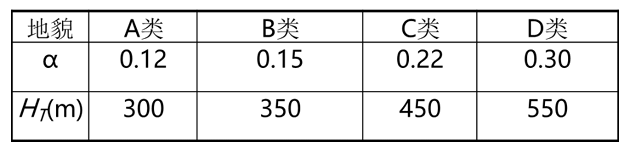
\includegraphics[width=0.5\textwidth]{../figure/3.png}
        \caption{地貌参数}
    \end{figure}

    死记硬背下公式,当然可以现场推导下:
    \[
    w_{0c} = w_{0s} \left( \frac{H_{Ts}}{z_s} \right)^{2\alpha_s} \left( \frac{H_{Tc}}{z_c} \right)^{-2\alpha_c}=0.45 \left( \frac{350}{10} \right)^{2 \times 0.15} \left( \frac{450}{10} \right)^{-2 \times 0.22} = 0.245 \,\mathrm{kN/m}^2
    \]
    于是,求得未知地区的标准风压后,计算其50m高度的风压:
    \[
    w_c = w_{0c} (\frac{50}{10})^{2 \times 0.22}=0.497\,\mathrm{kN/m}^2
    \]
    计算风速:
    \[
    w_c = \frac{1}{2} \rho v^2 = \frac{1}{2} \frac{\gamma}{g} v^2
    \]
    \[
    v = \sqrt{2 w_c g / \gamma} = \sqrt{0.497  / (1/1740)} = 29.4\,\mathrm{m/s}
    \]
\end{example}

\begin{example}
    已知:某矩形高层建筑,结构高度 $H=40\,\mathrm{m}$,平面长度 $D=30\,\mathrm{m}$,宽度 $B=25\,\mathrm{m}$,建造于城市市郊,地面粗糙度 $\alpha_a=0.22$,标准地貌的地面粗糙指数 $\alpha_s=0.15$,基本风压 $w_0=0.5\,\mathrm{kN/m}^2$。假设不考虑脉动风影响,沿高度均匀分成四段进行近似计算。求:顺风向风产生的建筑底部弯矩?

    \textbf{解:}

    1. 计算每段高度:
    \[
    \Delta h = \frac{H}{4} = \frac{40}{4} = 10\,\mathrm{m}
    \]
    各段中心高度分别为 $z_1=5\,\mathrm{m}$,$z_2=15\,\mathrm{m}$,$z_3=25\,\mathrm{m}$,$z_4=35\,\mathrm{m}$。

    2. 计算各段风压(采用风压高度变化系数):
    \[
    w(z) = \mu_s \mu_z(z) w_0
    \]
    其中 $\mu_s = 1.3 ,\text{是体型系数},\mu_z(z)=\left( \frac{H_{Ts}}{z_s} \right)^{2\alpha_s} \left( \frac{H_{Ta}}{z_a} \right)^{-2\alpha_a} \left( \frac{z}{z_s} \right)^{2\alpha_a} = 0.54 \times (\frac{z}{z_s})^{2 \times 0.22}$
    \begin{align*}
    w_1 &= 1.3 \times 0.54 \times (5/10)^{0.44} \times 0.5 = 0.26\,\mathrm{kN/m}^2 \\
    w_2 &= 1.3 \times 0.54 \times (15/10)^{0.44} \times 0.5 = 0.42\,\mathrm{kN/m}^2 \\
    w_3 &= 1.3 \times 0.54 \times (25/10)^{0.44} \times 0.5 = 0.52\,\mathrm{kN/m}^2 \\
    w_4 &= 1.3 \times 0.54 \times (35/10)^{0.44} \times 0.5 = 0.61\,\mathrm{kN/m}^2 \\
    \end{align*}
    3. 计算各段风荷载(作用面积 $A = B \times \Delta h = 25 \times 10 = 250\,\mathrm{m}^2$):
    \[
    F_i = w_i \cdot B \cdot \Delta h
    \]

    \begin{align*}
    F_1 &= 0.26 \times 250 = 65\,\mathrm{kN} \\
    F_2 &= 0.42 \times 250 = 105\,\mathrm{kN} \\
    F_3 &= 0.52 \times 250 = 130\,\mathrm{kN} \\
    F_4 &= 0.61 \times 250 = 152.5\,\mathrm{kN} \\
    \end{align*}
    4. 计算各段力臂(至底部距离):
    \begin{align*}
    l_1 &= 35\,\mathrm{m} \\
    l_2 &= 25\,\mathrm{m} \\
    l_3 &= 15\,\mathrm{m} \\
    l_4 &= 5\,\mathrm{m} \\
    \end{align*}

    5. 计算底部弯矩:
    \[
    M = \sum_{i=1}^{4} F_i \cdot l_i = 91.8 \times 35 + 148.5 \times 25 + 176.3 \times 15 + 197.5 \times 5
    \]
    \[
    = 3213 + 3712.5 + 2644.5 + 987.5 = 10557\,\mathrm{kN \cdot m}
    \]

    \textbf{答:} 顺风向风产生的建筑底部弯矩约为 $10557\,\mathrm{kN \cdot m}$。

\end{example}

\begin{example}
    什么情况下要考虑结构横风向风振效应?如何进行横风向风振验算?什么情况下要考虑结构横风向风振效应?如何进行横风向风振验算?

    当横向风作用引起结构共振时,结构横风向风振效应不可忽略。通过雷诺数验算。
\end{example}







\ifx\allfiles\undefined
\end{document}
\fi